\documentclass[12pt, letterpaper, twoside]{article}
\usepackage{nopageno,epsfig, amsmath, amssymb}
\usepackage{physics}
\usepackage{mathtools}
\usepackage{hyperref}
\usepackage{xcolor}
\hypersetup{
    colorlinks,
    linkcolor={blue},
    citecolor={blue},
    urlcolor={blue}
}
\usepackage{empheq}

\usepackage[letterpaper,
            margin=0.8in]{geometry}

\title{working out kick coordinates}
\author{\textbf{Tom Wagg}}

\newcommand{\question}[1]{{\noindent \it #1}}
\newcommand{\answer}[1]{
    \par\noindent\rule{\textwidth}{0.4pt}#1\vspace{0.5cm}
}
\newcommand{\todo}[1]{{\color{red}\begin{center}TODO: #1\end{center}}}

% custom function for adding units
\makeatletter
\newcommand{\unit}[1]{%
    \,\mathrm{#1}\checknextarg}
\newcommand{\checknextarg}{\@ifnextchar\bgroup{\gobblenextarg}{}}
\newcommand{\gobblenextarg}[1]{\,\mathrm{#1}\@ifnextchar\bgroup{\gobblenextarg}{}}
\makeatother

\newcommand{\avg}[1]{\left\langle #1 \right\rangle}
\newcommand{\angstrom}{\mbox{\normalfont\AA}}
\allowdisplaybreaks

\begin{document}

\section*{kick thoughts}

There's no way I'm going to get this right if I don't write it down haha. Okay so starting from COSMIC we are given the change in velocities due to kicks in the same coordinates system as BSE, which looks like this
\begin{center}
    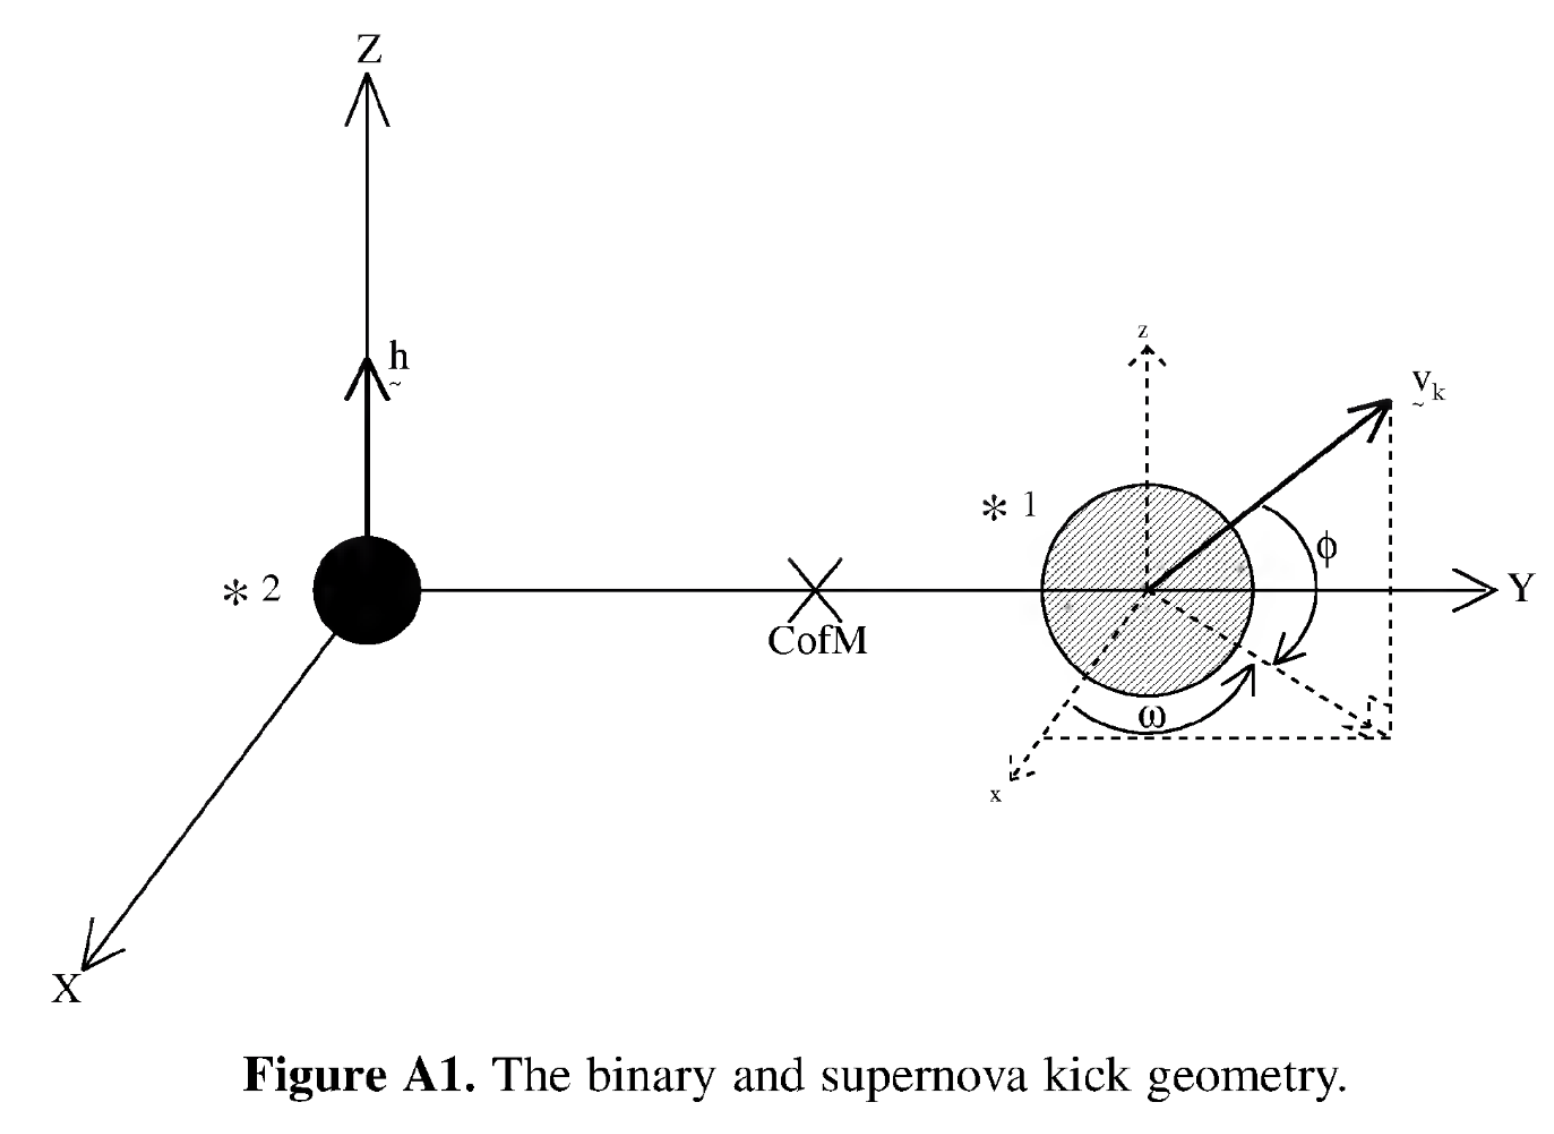
\includegraphics[width=0.5\textwidth]{static/bse_coordinates.png}
\end{center}
which means that the axes are defined as
\begin{itemize}
    \item \textbf{$x$-axis}: positive $x$ direction points in the direction of motion of the star that is \textit{not} going supernova
    \item \textbf{$y$-axis}: positive $y$ direction points from the non-supernova star to the supernova star
    \item \textbf{$x$-axis}: positive $z$ direction points in the direction of angular momentum vector of the system
\end{itemize}

We are given by COSMIC the change in systemic velocity, which I'm just going to call $\va{v}_{\rm kick}$ due to the kick in this coordinate system. This seems to account for the Blauuw kick and natal kick \textbf{but doesn't take the orbital motion into consideration}. Therefore, we need to add on the orbital motion of the supernova star $\va{v}_{\rm orb}$. From the definition of the coordinate system, this vector points along the negative $x$ axis, such that
\begin{equation}
    \va{v}_{\rm kick, eff} = \mqty[v_{\rm kick, x} - v_{\rm orb} \\ v_{\rm kick, y} \\ v_{\rm kick, z}]
\end{equation}
The orbital speed is calculated just as follows if we assume that the orbit is circular
\begin{equation}
    v_{\rm orb}^2 = \frac{G (M_1 + M_2)}{a}
\end{equation}
Now we just need to move this coordinate system into the Galactocentric frame so that we can add it to the system velocity, $v_{\rm sys}$. I \textit{think} that we consider this as basically a rotation about the $z$ and $x$ axis due to the random orbital phase and inclination to the Galactic plane respectively. Let's call these angles $\theta$ and $\phi$. In this case we can make a rotation matrix
\begin{align}
    \mathcal{R} &= \mqty[ \cos \theta & - \sin \theta & 0 \\ \sin \theta & \cos \theta & 0 \\ 0 & 0 & 1 ] \mqty[ 1 & 0 & 0 \\ 0 & \cos \phi & - \sin \phi \\ 0 & \sin \phi & \cos \phi ] \\
                &= \left[
                    \begin{array}{ccc}
                     \cos \theta & - \sin \theta \cos \phi & \sin \theta \sin \phi \\
                     \sin \theta & \cos \theta \cos \phi & -\cos \theta \sin \phi \\
                     0 & \sin \phi & \cos \phi \\
                    \end{array}
                    \right]
\end{align}
Which means that the final systemic velocity should be
\begin{equation}
    v_{\rm sys, final} = \mqty[v_{\rm sys, R} \\ v_{\rm sys, T} \\ v_{\rm sys, z}] + \mathcal{R} \cdot \va{v}_{\rm kick, eff},
\end{equation}
where
\begin{equation}
    \mathcal{R} \cdot \va{v}_{\rm kick, eff} = \left(
        \begin{array}{c}
         \cos \theta (v_{\rm kick, x}-v_{\rm orb})-v_{\rm kick, y} \sin \theta \cos \phi
           +v_{\rm kick, z} \sin \theta \sin \phi \\
         \sin \theta (v_{\rm kick, x}-v_{\rm orb})+v_{\rm kick, y} \cos \theta \cos \phi
           -v_{\rm kick, z} \cos \theta \sin \phi \\
         v_{\rm kick, y} \sin \phi+v_{\rm kick, z} \cos \phi \\
        \end{array}
        \right)
\end{equation}

\end{document}

 